% \documentclass[12pt]{article}
% \usepackage[frenchb]{babel}
% \usepackage{natbib}
% \usepackage[utf8]{inputenc}
% \usepackage[T1]{fontenc}
% \usepackage{tikz}
% \usepackage{amsmath}
% \usepackage{graphics}
% \usepackage{graphicx}
% \usepackage{url}
% \usepackage{psfrag}
% \usepackage{fancyhdr}
% \usepackage{vmargin}
% \usepackage[backend=biber]{biblatex}
% \usepackage{csquotes}
% \usepackage[hidelinks]{hyperref}
% \usepackage{enumitem}

% \pagestyle{fancy}


% \begin{document}
\subsubsection*{\large{Réunion d'équipe du 10 novembre 2020}}
    \addcontentsline{toc}{subsubsection}{Réunion d'équipe du 10 novembre 2020}
\begin{center}
\begin{tabular}{| l | l || c | c |}
    \hline
    Membres présents & Membres absents & Durée & Lieu \\
    \hline
    Mohamed-Omar CHIDA & & & \\ Mathis DUMAS & & 5h & Discord \\ Chaima TOUNSI OMEZZINE & & & \\ Céline ZHANG & & & \\
    \hline
\end{tabular}
\end{center}

\subsubsection*{Ordre du jour}
\begin{enumerate}
    \item Mise à niveau générale sur les connaissances du sujet
    \item Organisation du projet
    \item Installation des outils nécessaires au projet
    \item Découpage du sujet en tâches
    \item Planification des prochaines réunions
\end{enumerate}

\subsubsection*{Mise à niveau générale sur les connaissances du sujet}
Nous avons mis en commun nos connaissances concernant le sujet, partagé nos documentations, et expliqué les notions ambigües, suivi d'une présentation de nos préférences ou nos points forts respectives.

\subsubsection*{Organisation du projet}
Nous avons parlé du sens de déroulement général du projet (quand faire les documentations, les premières lignes, quand aborder quelles parties, quand commencer la rédaction de rapport, etc.), en abordant également la gestion de projet (les stratégies, les rôles, voir le tableau~\ref{tab:roles}, les facilités, les difficultés par la matrice de SWOT, voir figure~\ref{fig:Matrice SWOT}), et puis nous avons parlé de la structure de nos dépôts, nos dossiers, nos codes, notre rapport (en définissant les styles, les normes, etc.). Nous adoptons la gestion SCRUM, qui utilise la méthode du \textsl{sprint} \footnotemark \ pour réaliser les travaux.
    \begin{center}
        \begin{tabular}{|l|l|}
        \hline
            Membre de l'équipe 13 & Rôles ou charges \\
        \hline
        \hline
            Mohamed-Omar CHIDA & leader \\
        \hline
            Mathis DUMAS & documentation \\
        \hline
            Chaima TOUNSI OMEZZINE & reviewer \\
        \hline
            Céline ZHANG & organisateur \\
        \hline
        \end{tabular}\\
        %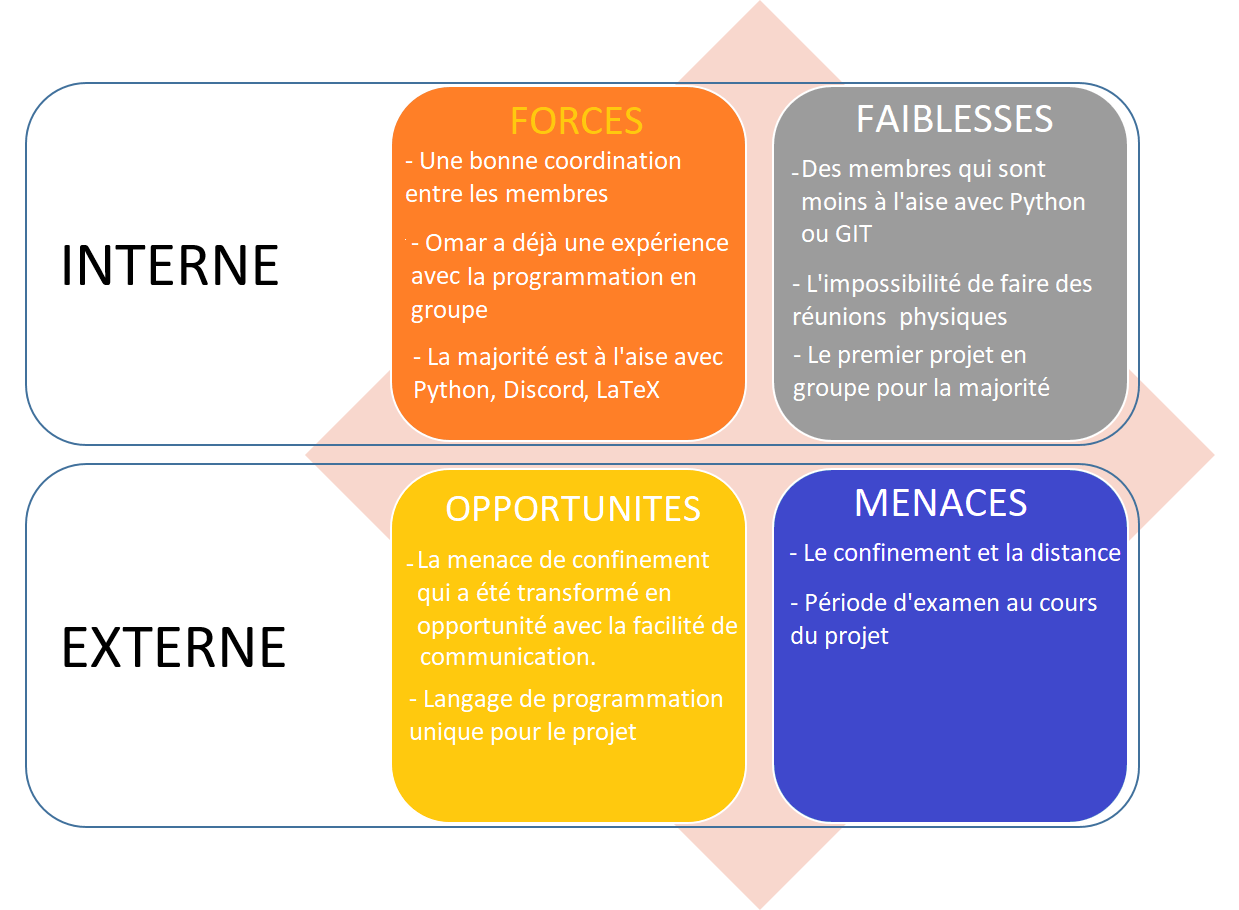
\includegraphics[scale = 0.45]{Images/Gestion de Projet/Matrice_swot.png}
    \end{center}


\footnotetext{Méthode d'organisation de travail d'équipe qui consiste à se fixer des tâches pour un cycle (1 à 2 semaines) et de les finir avant la fin de celle-ci.}

\subsubsection*{Installation des outils nécessaires au projet}
La présentation des outils utilisables et les outils nécessaires est primordiale pour commencer à travailler. Nous avons donc présenté les outils à disposition, créé nos dossiers et fichiers dans le dépôt, installé les logiciels.

\subsubsection*{Découpage du sujet en tâches}
En utilisant le tableau de bord Trello\footnotemark \ nous avons découpé le cahier de charge en tâches nécessaires à la réalisation du livrable final. Ce qui nous permettra aussi de surveiller l'avancer de chacun sur ses tâches.
\footnotetext{Outil qui nous permet de planifier en ligne des activités. \ref{fig:Trellomilieu}}

\subsubsection*{Planification des prochaines réunions}
Nous décidons de faire en général une réunion par semaine (flexible suivant les disponibilités), qui sera tous les samedis à 18h00 sur Discord, bien sûr il peut y avoir des sortes de stand-up-meeting en appel pour régler les soucis ou prendre des nouvelles (le tableau Trello permet aussi de laisser des messages pour indiquer les problèmes et demander de l'aide).

\paragraph{\emph{TO-DO LIST}}
\begin{itemize}
    \item Se documenter (si nécessaire) et réfléchir à la première partie du sujet concernant les notions de descriptions du SARS-COV2
    \item Commencer à écrire les lignes de codes pour la première partie
    \item Envoyer un mail M. Festor pour demander la langue à utiliser pour les commentaires
\end{itemize}

\emph{Prochaine réunion : 14/11/2020}\\

% \end{document}